\documentclass[journal]{IEEEtran}

\usepackage{amsmath}
\usepackage{amsfonts}
\usepackage{amssymb}
\usepackage{amsthm}
%\setcounter{MaxMatrixCols}{20} % needed for wide adjoints

\usepackage{mathdots} % for \iddots

\usepackage{tikz}
\usetikzlibrary{matrix}
\usetikzlibrary{calc}
\tikzset{node style ge/.style={circle}}

\usepackage{array}

\usepackage{graphicx}

%\usepackage{hyperref}

\newcommand{\opn}[1]{\operatorname{#1}}
\newcommand{\reals}{\mathbb{R}}
\newcommand{\defeq}{\mathrel{\mathop:}=}

%TODO should this be a ``lecture note'' or a ``tips and tricks''?

\begin{document}
%\title{Fast Computation of the Discrete Adjoint Wavelet Transform}
\title{Application of Adjoint Operators in Gradient Computations}
\author{James~Folberth and 
        Stephen~Becker%
\thanks{J. Folberth and S. Becker are with the Department
of Applied Mathematics, University of Colorado at Boulder,
Boulder, CO, 80309 USA}}

\markboth{IEEE Signal Processing Magazine: Lecture Notes}%
{J. Folberth and S. Becker: Fast Adjoint Wavelet}

\maketitle

% For IEEE, Don't use math or other special symbols; greek probably okay.
\begin{abstract}
   When using first-order optimization algorithms, it is often the case that the user must supply the gradient of the differentiable terms in the objective function.  We consider two example problems that have a Euclidean error term involving a linear operation on the problem variables.  The gradient of the Euclidean error term involves both the linear operator and its adjoint, which, in our examples, is not known in the literature.  The first example is an image deblurring problem, where the linear operation is multi-stage wavelet synthesis.  Our formulation of the adjoint holds for a variety of boundary conditions, which allows the formulation to generalize to a larger class of problems.  The second example is a blind channel estimation problem taken from the convex optimization literature; the linear operation is convolution, but with a slight twist.  In each example, we show how the adjoint operator can be applied efficiently.
\end{abstract}

\subsection*{Prerequisites}
The reader should be familiar with linear algebra, wavelets, and basic Fourier analysis.  Knowledge of first-order iterative optimization algorithms is beneficial for motivating the fast adjoint computation, but should not be necessary to understand the adjoint computation itself.  We begin by briefly motivating the need for a fast adjoint operator and then turn toward the two examples.\\


%TODO Not sure what to call this section
%TODO How do we cite Vandenberghe's course notes? http://www.seas.ucla.edu/~vandenbe/ee236c.html
\section{A Generic Optimization Problem}
% [[[
In this lecture note we consider as examples a few variants of the optimization problem

\begin{equation}
\label{eq:model_problem}
\min_x ~\frac{1}{2}\|\mathcal{A}x-b\|_2^2 + \lambda \|x\|_1,
\end{equation}

\noindent where $\mathcal{A}$ is a linear operator, $\|\cdot\|_2$ is the $\ell_2$ norm, and $\|\cdot\|_1$ is the $\ell_1$ norm.  Loosely speaking, we pose this problem to attempt to find an $x$ such that $\mathcal{A}x$ is close to $b$, but also such that $x$ is sparse.  This problem usually comes up when we try to discover an unknown signal $x$ from an observed signal $b$, subject to some structural information about the unknown signal $x$ (sparsity, in this case).\\

\noindent Let $g(x) = \frac{1}{2}\|\mathcal{A}x-b\|_2^2$ and $h(x)=\lambda \|x\|_1$.  Notice that $g(x)$ is convex and differentiable, and $h(x)$ is convex but non-differentiable.  The scalarization parameter $\lambda$ controls the relative importance of the approximation error $g(x)$ and the sparsity heuristic $\|x\|_1$.  Loosely speaking, larger $\lambda$ should yield a sparser solution.\\

Even though $h(x)$ is non-differentiable, there exist many efficient algorithms for solving the above problem and its variants.  Popular methods include the proximal gradient method and its variants, which include iterative shrinkage thresholding and projected gradient.  Crucial to the speed of these methods is an efficient proximal mapping (prox-operator) for the non-differentiable term $h(x)$.  The proximal mapping is defined as

\[ \opn{prox}_h(x) = \opn{argmin}_{y} \left(h(y) + \dfrac{1}{2}\|y-x\|_2^2\right). \] 

\noindent The proximal mapping can be thought of as finding the point minimizing $h(y)$ plus a simple quadratic model about the point $x$.  For $h(y) = \|y\|_1$, the proximal mapping is the shrinkage (``soft-threshold'') operator and takes the following particularly simple form:

\[ \opn{prox}_h(x) = \left\{\begin{array}{ll} x_i - 1 & x_i \ge 1\\ 0 & |x_i| < 1\\ x_i + 1 & x_i \le 1.\end{array}\right. \]

\noindent The main step of a simple proximal gradient method is

\[ x^{(k)} = \opn{prox}_{t_k h}\left(x^{(k-1)} - t_k \nabla g(x^{(k-1)})\right), \] 

\noindent with step size $t_k>0$.  The reader may note that this update resembles the simple gradient descent update for minimizing $g(x)$, with the exception of the proximal mapping which handles the non-differentiable term $h(x)$.  It is clear that an efficient proximal mapping is desired, as the proximal mapping must be evaluated at each step of the simple proximal gradient method.\\

The gradient of the differentiable term $g(x)$ is found to be

\[ \nabla g(x) = \mathcal{A}^\ast(\mathcal{A}x-b). \] 

\noindent It is during the evaluation of the gradient $\nabla g(x)$ that we need efficient means of computing the action of $\mathcal{A}$ and its adjoint $\mathcal{A}^\ast$.  As we will see in the next sections, the operator $\mathcal{A}$ tends to have a well known, efficient forward and (pseudo)inverse transform (e.g. discrete cosine transform, discrete wavelet transform).  For unitary and orthogonal operators, the adjoint is identically the inverse.  For non-unitary and non-orthogonal operators, however, applying the adjoint efficiently may pose a problem.  The following examples show cases where a fast adjoint operation is possible.

% ]]]

\section{Example 1: An Image Deblurring Problem}
% [[[
Digital images can be blurred through a variety of means.  For example, the optical system can be out of focus and atmospheric turbulence can cause blurring of astronomical images.  The goal of image deblurring is to recover the original, sharp image by posing the blurring process in a mathematical model.\\

In this example, we use the formulation used in \cite{beck_2009}.  It is assumed that the blurring action is known, and the deblurring problem is posed as an optimization problem, where the optimization variables are the wavelet coefficients of the recovered image.  Let $\mathcal{R}$ be a known blurring operator.  For instance, $\mathcal{R}$ could represent a Gaussian point spread function (PSF) under symmetric (reflexive) boundary conditions \cite{hansen_2006}.  Again, this model assumes that we have a good model of the blurring operator.\\

Let $\mathcal{W}$ represent a multi-level wavelet synthesis operator with suitable boundary conditions.  Let $b$ be the observed, blurry image.  Let $\mathcal{A}=\mathcal{RW}$ be the linear operator that synthesizes an image from wavelet coefficients $x$ and then blurs the synthesized image under the blurring operator $\mathcal{R}$.  The image deblurring task is now readily posed as the optimization problem (\ref{eq:model_problem}), where we seek to recover sparse wavelet coefficients that accurately reconstruct the blurred image:

\begin{equation}
\label{eq:syn_problem}
\min_x~ \dfrac{1}{2}\|\mathcal{RW}x-b\|_2^2 + \lambda \|x\|_1,
\end{equation}

\noindent From the sparse wavelet coefficients in an optimal solution $\hat{x}$, we can synthesize the deblurred image via $\mathcal{W}\hat{x}$.  This formulation is sometimes called the \emph{synthesis} formulation, since we synthesize an image from the wavelet coefficients in the optimization variable $x$.\\

The gradient of the differentiable term ${g(x)=\frac{1}{2}\|\mathcal{RW}x-b\|_2^2}$ is

\[ \nabla g(x) = \mathcal{W}^\ast \mathcal{R}^\ast(\mathcal{RW}x-b). \] 

\noindent In the case of a blurring PSF, we can apply $\mathcal{R}$ and $\mathcal{R}^\ast$ efficiently in the Fourier domain via the FFT \cite{beck_2009, hansen_2006}.  Wavelet software packages (e.g. {\sc matlab} Wavelet Toolbox \cite{matlab_wt_2015}) implement fast discrete wavelet analysis and synthesis, which correspond to $\mathcal{W}^\dagger$ and $\mathcal{W}$ (we use $\mathcal{A}^\dagger$ to denote the Moore-Penrose pseudoinverse of $\mathcal{A}$).  However, the adjoint wavelet transform is not implemented in software packages and is not discussed in the literature.\\
%TODO how do we cite "the adjoint transform is not discussed"?


\subsection{The adjoint for orthogonal wavelets}
There is hope, however!  For orthogonal wavelets (e.g. Haar and more generally Daubechies wavelets), the pseudoinverse $\mathcal{W}^\dagger$ is identically the adjoint $\mathcal{W}^\ast$, subject to matching boundary conditions, so the adjoint operator can be evaluated via the analysis operator $\mathcal{W}^\dagger$.  Thus, one can compute the gradient as

\[ \nabla g(x) = \mathcal{W}^\dagger \mathcal{R}^\ast \left(\mathcal{RW}x-b\right). \] 

\noindent Beck and Teboulle did exactly this with a three-stage discrete Haar wavelet transform \cite{beck_2009}.  For an example image, consider the cameraman image, shown in Figure \ref{fig:cameraman_original}.  We prescribe symmetric boundary conditions on the image, which will affect both $\mathcal{W}$, $\mathcal{R}$, and their adjoints.  Symmetric boundary conditions (compared to periodic or zero-padded boundary conditions) produce significantly less edge effects, and so are a natural choice.  Luckily, for orthogonal wavelets, the adjoint of $\mathcal{W}$ with symmetric boundary conditions is identically the inverse $\mathcal{W}^\dagger=\mathcal{W}^{-1}$ with symmetric boundary conditions, so one can use existing wavelet libraries without hassle, e.g. \cite{matlab_wt_2015}.\\
%TODO do existing wavelet libraries actually do the extension pinv adjoint correctly?
%     No, but the extension operator is "close" to the extension pinv adjoint, so it's approx correct.
%     For zero-padding, the extension pinv is identically the adjoint.

\begin{figure}
   \centering
   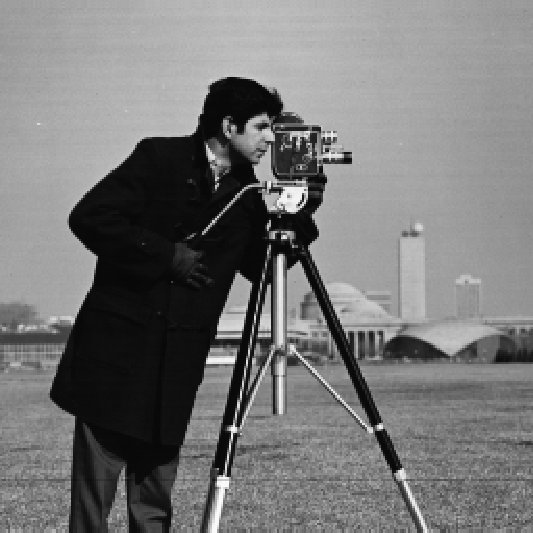
\includegraphics[width=0.8\columnwidth]{figures/cameraman.pdf}
   \caption{The original, unblurred cameraman image.  To create the blurred image, the $\mathcal{R}$ is applied to the original image and Gaussian noise is added.}
   \label{fig:cameraman_original}
\end{figure}

Figure \ref{fig:cameraman_200_db1_sym} shows the deblurred image after 200 iterations of FISTA, a fast proximal gradient method, developed by Beck and Teboulle \cite{beck_2009}.  The wavelet synthesis operator $\mathcal{W}$ is taken to be a three-stage Haar discrete wavelet transform with symmetric boundary conditions.  In this case, the operator $\mathcal{W}$ is orthogonal, so $\mathcal{W}^\ast = \mathcal{W}^\dagger$, which is the three-stage wavelet reconstruction operation with symmetric boundary conditions.  So, coding up the adjoint transform is a simple matter of performing the analysis operation with suitable boundary conditions.

\begin{figure}
   \centering
   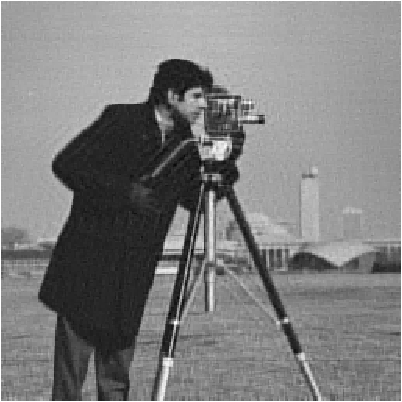
\includegraphics[width=0.8\columnwidth]{figures/cameraman_rec_200_db1_sym_trim.pdf}
   \caption{Deblurred image after 200 iterations of FISTA with $\mathcal{W}$ a three-stage Haar transform with symmetric boundary conditions.}
   \label{fig:cameraman_200_db1_sym}
\end{figure}


\subsection{The adjoint for biorthogonal wavelets}
For biorthogonal wavelets, we no longer have $\mathcal{W}^\ast=\mathcal{W}^\dagger$.  Since we have relaxed ourselves to biorthogonal wavelets, it is perhaps too much to ask that the adjoint of the primal wavelet synthesis operator involves only the primal wavelets.  Let us recall briefly the pertinent aspects of frames of Hilbert spaces.  These facts are described in more detail in \cite{mallat_2009}.\\

Let $\mathcal{H}$ be a Hilbert space and take $f\in\mathcal{H}$ to be an arbitrary vector in the Hilbert space.  Let $\{\phi_n\}_{n\in\Gamma}$, where $\Gamma$ is an index set, be a set of vectors in $\mathcal{H}$.  The set of vectors $\{\phi_n\}_{n\in\Gamma}$ is called a frame of $\mathcal{H}$ if there exists constants $B\ge A > 0$ such that

\[ \forall f\in \mathcal{H}, \quad A\|f\|^2 \le \sum_{n\in\Gamma} |\langle f,\phi_n\rangle|^2\le B \|f\|^2. \] 

\noindent If the set $\{\phi_n\}_{n\in\Gamma}$ is a frame and is linearly independent, we call it a Riesz basis.\\

We assume henceforth that the set $\{\phi_n\}_{n\in\Gamma}$ is a frame of $\mathcal{H}$ with bounds $B\ge A > 0$.  We can define the frame analysis operator $\Phi$ via

\[ \forall n\in \Gamma,\quad \Phi f[n] = \langle f,\phi_n\rangle. \] 

\noindent The frame analysis operator computes the expansion coefficients of $f$ in the frame $\{\phi_n\}_{n\in\Gamma}$.  The frame synthesis operator is $\Phi^\ast$, and constructs a vector in $\mathcal{H}$ given expansion coefficients.  Since $\{\phi_n\}_{n\in\Gamma}$ is assumed to be a frame, $\Phi^\ast\Phi$ is invertible, and we may define the Moore-Penrose pseudoinverse $\Phi^\dagger$, which implements reconstruction, as $\Phi^\dagger = \left(\Phi^\ast\Phi\right)^{-1}\Phi$.\\

Reconstruction with the pseudoinverse of the frame operator can be thought of as synthesis with a dual frame.  The dual frame analysis operator and dual frame vectors are defined via

\[ \forall n\in \Gamma, \quad \tilde{\Phi}f[n] = \langle f,\tilde{\phi}_n\rangle, \quad \text{where } \tilde{\phi}_n = \left(\Phi^\ast\Phi\right)^{-1}\phi_n. \] 

\noindent Then the dual frame synthesis operator satisfied $\tilde{\Phi}^\ast = \Phi^\dagger$.  Notice that we also have $\Phi^\ast = \tilde{\Phi}^\dagger$; this relation provides the basic idea for computing the adjoint of the discrete wavelet synthesis operator $\mathcal{W}$.  Ignoring boundary effects and selecting the biorthogonal wavelets so that $\Phi^\dagger=\mathcal{W}$, we have the following:

\begin{align*}
   \mathcal{W}^\ast &= \left(\Phi^\dagger\right)^\ast = \left(\left(\Phi^\ast\Phi\right)^{-1}\Phi^\ast\right)^\ast = \Phi\left(\Phi^\ast\Phi\right)^{-1}\\ 
                    &= \left(\Phi^\ast\right)^\dagger = \left(\tilde{\Phi}^\dagger\right)^\dagger\\
                    &= \tilde{\Phi},
\end{align*}

\noindent where we have used various properties of the pseudoinverse.  Thus, ignoring boundary conditions, the adjoint of wavelet synthesis is dual wavelet analysis!  Note that in the case of orthogonal wavelets, $\Phi^\ast\Phi$ is the identity, the dual frame is identically the primal frame, and ${\mathcal{W}^\ast = \tilde{\Phi}=\Phi=\mathcal{W}^\dagger}$, exactly as before.\\

It now remains to include boundary conditions.  A standard method for imposing boundary conditions on finite, discrete signals is to extend the signal to match those boundary conditions and perform the wavelet operations on the extended signal, assuming zero boundary conditions for the extended signal; this is the approach used in {\sc matlab}'s Wavelet Toolbox \cite{matlab_wt_2015}.  If we let $\mathcal{E}$ be the extension operator and $\mathcal{W}^\dagger_\text{zpd}$ be the wavelet analysis operator for extended signals under zero boundary conditions, we can write wavelet analysis as 
%TODO motivate why we use W_zpd better

\[ \mathcal{W}^\dagger = \mathcal{W}^\dagger_\text{zpd}\mathcal{E}. \] 

\noindent This separation of signal extension and wavelet operations provides a nice framework for determining the adjoint:

\[ \mathcal{W} = \mathcal{E}^\dagger\mathcal{W}_\text{zpd}, \quad \mathcal{W}^\ast = \mathcal{W}^\ast_\text{zpd}(\mathcal{E}^\dagger)^\ast. \] 

Consider a signal $y[n]$, $n=0,...,N-1$.  Let $L_p$ be the length of the wavelet analysis filters (one can zero-padd a shorter filter to length $L_p$).  The double sided zero-padded extension of $y[n]$ puts $L_p-1$ zeros on each end of the signal:
\[ \underbrace{0, ..., 0}_{L_p-1}, y[0], ..., y[N-1], \underbrace{0, ..., 0}_{L_p-1}. \]

\noindent We can write down the linear operator $\mathcal{E}_\text{zpd}$ as a matrix that performs this operation on $y[n]$.

\[ \mathcal{E}_\text{zpd} = \begin{bmatrix} 0_{(L_p-1)\times N}\\ I_{N\times N}\\ 0_{(L_p-1)\times N}\end{bmatrix} = \begin{bmatrix} 0 & 0 & \cdots & 0 & 0\\ \vdots & \vdots &\ddots & \vdots & \vdots\\ 0 & 0 & \cdots & 0 & 0\\[0.5em] 1 & 0 & \cdots & 0 & 0\\ 0 & 1 & \cdots & 0 & 0\\ \vdots & \vdots & \ddots & \vdots & \vdots\\ 0 & 0 & \cdots & 1 & 0\\ 0 & 0 & \cdots & 0 & 1\\[0.5em] 0 & 0 & \cdots & 0 & 0\\ \vdots & \vdots & \ddots & \vdots & \vdots\\ 0 & 0 & \cdots & 0 & 0\end{bmatrix}. \] 

\noindent Once we have this explicit form of $\mathcal{E}_\text{zpd}$, we can find the adjoint of its pseudoinverse.  In this case we have that $\left(\mathcal{E}_\text{zpd}^\dagger\right)^\ast = \mathcal{E}_\text{zpd}$.  Although the zero-padded extension is simple to work with, it is not usually a reasonable extension mode for practical applications.  A better extension mode is the half-point symmetric extension, which is the default extension mode in {\sc matlab}'s Wavelet Toolbox \cite{matlab_wt_2015}.\\

The double sided half-point symmetric extension reflects the signal about its boundaries in the following manner:

\[ \underbrace{y[L_p-1], ..., y[0]}_\text{Left extension}, y[0], ..., y[N-1], \underbrace{y[N-1], ..., y[N+L_p-2]}_\text{Right extension}. \] 

\noindent As in the zero-padded case, we can readily form a matrix that performs this operation on $y[n]$.

\[ \mathcal{E}_\text{sym} = \begin{bmatrix} & & \iddots & & &\\ & 1 &&&&\\ 1&&&&&\\1&&&&\\&1&&&&\\&&\ddots&&&\\&&&1&\\&&&&1\\&&&&1\\&&&1&\\&&\iddots&&\end{bmatrix}. \]

\noindent The adjoint of the pseudoinverse can be computed in closed form and essentially amounts to rescaling the nonzero entries of $\mathcal{E}_\text{sym}$.  Assuming $N > 2(L_p-1)$, which usually occurs in practice, the adjoint of the  pseudoinverse of $\mathcal{E}_\text{sym}$ is 

\[ \left(\mathcal{E}_\text{sym}^\dagger\right)^\ast = \begin{bmatrix} & \iddots \\ 1/2&&&&&\\1/2&&&&\\&\ddots&&&&&&\\&&1/2&\\&&&1\\&&&&\ddots\\&&&&&1\\&&&&&&1/2\\&&&&&&&\ddots\\&&&&&&&&1/2\\&&&&&&&&1/2\\&&&&&&&\iddots\\\end{bmatrix}. \]

\noindent If $N \le 2(L_p-1)$, the form of the pseudoinverse is slightly different, with some of the $1/2$ terms becoming $1/3$; both cases are considered in our implementation.\\


\begin{figure}
   \centering
   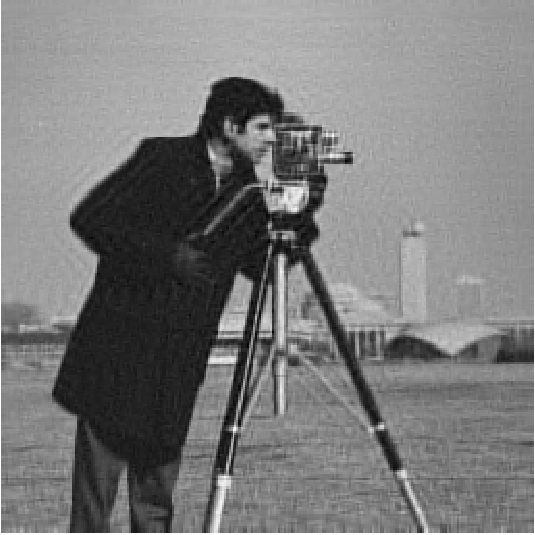
\includegraphics[width=0.8\columnwidth]{{figures/cameraman_rec_200_bior4.4_sym_trim}.pdf}
   \caption{Deblurred image after 200 iterations of FISTA with $\mathcal{W}$ a three-stage CDF 9/7 transform with symmetric boundary conditions.}
   \label{fig:cameraman_200_bior4.4_sym}
\end{figure}

Figure \ref{fig:cameraman_200_bior4.4_sym} shows the deblurred cameraman image after 200 iterations of FISTA using a three-stage CDF 9/7 transform with symmetric boundary conditions.
%TODO comment on sparsity levels of db1 vs bior4.4?  That's not really a fair comparison...



%TODO include this section too (but beware: it's old!)
%TODO briefly mention P. Combettes one theorem regarding unequivalence of analysis and synthesis formulation
%     for nonorthogonal transforms (and how the proximal mapping plays into why).
%\subsection{Analysis Formulation}
%We note here that there is an alternative formulation of the image deblurring problem.  The formulation (\ref{eq:syn_problem}), where $x$ is a vector of wavelet coefficients, is called the synthesis form.  We can also consider the problem in analysis form:
%
%\begin{equation}
%\label{eq:ana_form}
%\min_y~ \|\mathcal{R}y-b\|_2^2 + \lambda \|\mathcal{W}^\dagger y\|_1.
%\end{equation}
%
%\noindent We use $\mathcal{W}^\dagger$ to denote the Moore-Penrose pseudoinverse of $\mathcal{W}$; this is the standard operation of wavelet analysis.  In the analysis form, the optimization variable $y$ is an image.  An optimal solution $y^\ast$ should be a good approximation of the original, sharp image.\\
%
%If the wavelet synthesis operator is orthogonal, so that ${\mathcal{W}^\ast=\mathcal{W}^\dagger=\mathcal{W}^{-1}}$, we then have ${x=\mathcal{W}^{-1}y}$.  Moreover, the synthesis and analysis formulations are equivalent, in the sense that an optimal solution of one formulation is readily obtained from an optimal solution of the other.\\

%Wavelet software packages (e.g. \cite{matlab_wt_2015}) implement fast wavelet analysis and synthesis operators, which we can apply to 

% ]]]

%TODO might have to cut this out if the problem doesn't recover things well
%TODO perhaps introduce problem as min \sum_i \|x_i - h_i\ast s\|_2^2 + \|h_i\|_1 + \|s\|_1
%     then introduce the linear operator \mathcal{A}
\section{Example 2: Blind Channel Estimation}
% [[[
Another application where an interesting adjoint is involved in the gradient computation is in blind channel estimation.  In blind channel estimation, a single source sends an unknown signal over multiple channels with unknown response.  Observers collect the output of each channel and collectively attempt to determine the source signal and the channel impulse response from each channel.  Let $s$ be the unknown source signal of length $N$ and $h_i$ the channel impulse response of the $i$th channel, each of length $K$.  Then the output of the $i$th channel is

\[ x_i = h_i\ast s, \] 

\noindent and will be of length $K+N-1$.  We hope to recover the source $s$ and channel responses $h_i$ from the output signals $x_i$.   However, note that there is both a magnitude and phase ambiguity in $h_i$ and $s$, since we can multiply $h_i$ by $\alpha\neq 0$ and divide $s$ by $\alpha$, leaving $x_i$ unchanged.\\

Recently Ahmed et al. \cite{ahmed_2013} published a paper considering blind deconvolution via convex optimization.  Crucial to their method, which is based on low-rank recovery, is the following observation: the convolution $h_i\ast s$ can be formed as a linear operation on the elements of the rank-1 matrix $h_is^T$:

\[ h_i\ast s = \mathcal{A}(h_is^T). \] 

\noindent The operation $x_i=\mathcal{A}(h_is^T)$ acts on the $K\times N$ matrix $h_is^T$ by summing each antidiagonal, producing an element of $x_i$.  This action is illustrated in Figure \ref{fig:action_of_A}.\\

For simplicity, let's assume we have a single channel $h$ with observed output $x$.  Using the convolution operator $\mathcal{A}$, we can pose the recovery problem as

\[ \min_{h,s}~ \|\mathcal{A}(hs^T)-x\|_2^2 + \lambda_h\|h\|_1 + \lambda_s \|s\|_1, \] 

\noindent where we include the terms $\lambda_h\|h\|_1$ and $\lambda_s\|s\|_1$ to promote sparsity in the recovered signals.  To promote other structure in the recovered signals (assuming it is present in the true signals), we can in principle include other terms, such as $\lambda_h\|h\|_{TV}$, the total-variation norm.  Note that since this problem involves quadratic terms in $hs^T$, it is a non-convex problem.\\

The gradients of the differentiable $\ell_2$ error term $g(h,s)=\|\mathcal{A}(hs^T)-x\|_2^2$ are

\begin{align*}
   \nabla_h g &= \left[\mathcal{A}^\ast\left(A(hs^T) - x\right)\right]s\\
   \nabla_s g &= \left[\mathcal{A}^\ast\left(A(hs^T) - x\right)\right]^Th.
\end{align*}

\begin{figure}
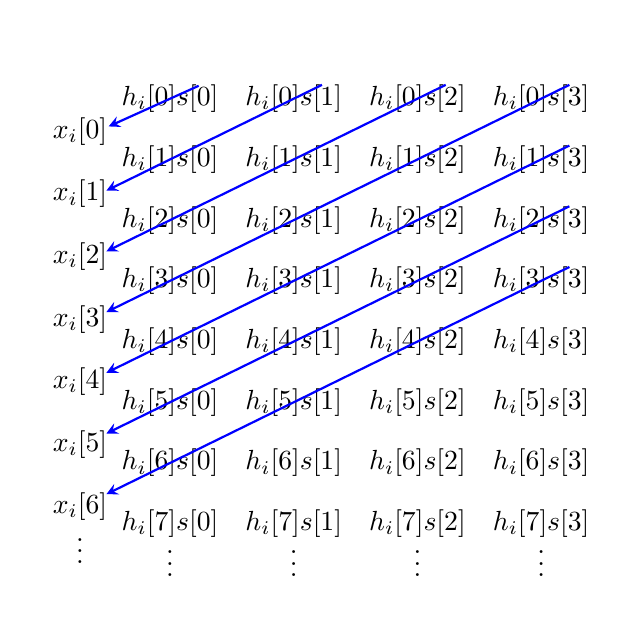
\begin{tikzpicture}[baseline=(hs.center)]
   % [[[
   % based on figure from Romberg et al. "Multichannel blind deconvolution..."
   % and examples from http://www.texample.net/tikz/examples/mnemonic-rule-for-matrix-determinant/
   % http://tex.stackexchange.com/questions/83046/position-two-stacked-tikz-matrices
   % http://www.texample.net/tikz/examples/energy-level-diagram/
   \matrix (hs) [matrix of math nodes, nodes = {node style ge},, column sep=0mm, row sep=-8mm]
   {h_i[0]s[0] & h_i[0]s[1] & h_i[0]s[2] & h_i[0]s[3] \\
    h_i[1]s[0] & h_i[1]s[1] & h_i[1]s[2] & h_i[1]s[3] \\
    h_i[2]s[0] & h_i[2]s[1] & h_i[2]s[2] & h_i[2]s[3] \\
    h_i[3]s[0] & h_i[3]s[1] & h_i[3]s[2] & h_i[3]s[3] \\
    h_i[4]s[0] & h_i[4]s[1] & h_i[4]s[2] & h_i[4]s[3] \\
    h_i[5]s[0] & h_i[5]s[1] & h_i[5]s[2] & h_i[5]s[3] \\
    h_i[6]s[0] & h_i[6]s[1] & h_i[6]s[2] & h_i[6]s[3] \\
    h_i[7]s[0] & h_i[7]s[1] & h_i[7]s[2] & h_i[7]s[3] \\
    \vdots & \vdots & \vdots & \vdots\\
   };

   \begin{scope}[xshift=-35mm,yshift=-2.5mm]
   %TODO need to hack these offsets and spacits correctly
   \matrix (y) [matrix of math nodes, nodes = {node style ge},, column sep=0mm, row sep=-3mm]
   {x_i[0]\\
    x_i[1]\\
    x_i[2]\\
    x_i[3]\\
    x_i[4]\\
    x_i[5]\\
    x_i[6]\\[-2mm]
    \vdots\\
   };
   \end{scope}

   \draw [thick,->,>=stealth,shorten >=4mm,shorten <=-4mm,color=blue] (hs-1-1.center) to ($(y-1-1.center) + (0mm,-1mm)$); % this is a hack, but it's quite close
   \draw [thick,->,>=stealth,shorten >=-9mm,shorten <=-4mm,color=blue] (hs-1-2.center) to (hs-2-1.center);
   \draw [thick,->,>=stealth,shorten >=-9mm,shorten <=-4mm,color=blue] (hs-1-3.center) to (hs-3-1.center);
   \draw [thick,->,>=stealth,shorten >=-9mm,shorten <=-4mm,color=blue] (hs-1-4.center) to (hs-4-1.center);
   \draw [thick,->,>=stealth,shorten >=-9mm,shorten <=-4mm,color=blue] (hs-2-4.center) to (hs-5-1.center);
   \draw [thick,->,>=stealth,shorten >=-9mm,shorten <=-4mm,color=blue] (hs-3-4.center) to (hs-6-1.center);
   \draw [thick,->,>=stealth,shorten >=-9mm,shorten <=-4mm,color=blue] (hs-4-4.center) to (hs-7-1.center);
   % ]]]
\end{tikzpicture}
\caption{How $x_i$ is formed via $\mathcal{A}(h_is^T)$.  Adapted from \cite{romberg_2013}.}%TODO
\label{fig:action_of_A}
\end{figure}

\noindent The operator $\mathcal{A}$ is a little bit strange in that it maps matrices to vectors, so its adjoint is not quite obvious (i.e. we cannot directly compute the conjugate transpose of $\mathcal{A}$), but we do know that the adjoint maps vectors to matrices.  This fact is apparent in $\nabla_sg$, where we must compute a matrix-vector product with the matrix transpose of $\mathcal{A}^\ast\left(\mathcal{A}(hs^T)-x\right)$.  Note that the matrix transpose of $\mathcal{A}^\ast(\cdot)$ is different than applying another adjoint to $\mathcal{A}^\ast$.\\

To find the adjoint, we can directly apply the defining relation for the adjoint.  We consider an arbitrary matrix $X\in\reals^{K\times N}$ and vector $y\in\reals^{K+N-1}$.  The adjoint is defined via

\begin{equation}
   \label{eq:A_adjoint_def}
   \left\langle \mathcal{A}(X),y \right\rangle = \left\langle X, \mathcal{A}^\ast(y)\right\rangle \quad \forall X,y.
\end{equation}

\noindent Note that the inner product on the left-hand side of equation \ref{eq:A_adjoint_def} is the usual vector inner product on $\reals^{K+N-1}$, while the inner product on the right-hand side is the usual matrix inner product on $\reals^{K\times N}$.  We can explicitly write down $\mathcal{A}(X)$ and expand the vector inner product.

\[ \left\langle \mathcal{A}(X),y\right\rangle = \sum_{k=0}^{K+N-2}y[k] \left(\sum_{n=n_1(k)}^{n_2(k)} X[n,k-n]\right) \] 

\noindent where we have defined the bounds $n_1(k) = {\max\{0,k+1-N\}}$ and $n_2(k) = {\min\{K-1,k\}}$.  If $X=h_is^T$, then the inner summation computes the $k$th term of the convolution $h_i\ast s$.  We can expand the first few terms of the vector inner product and keep track of the terms multiplying $y[k]$.

\begin{align*}
   \left\langle\mathcal{A}(X),y\right\rangle &= y[0]X[0,0] + y[1]\left(X[0,1]+X[1,0]\right)\\
                                             &\,+ y[2]\left(X[0,2] + X[1,1] + X[2,0]\right) + \cdots.\\
\end{align*}

\noindent Now notice that $X[k,n]$ is always multiplied by $y[k+n]$.  This means that we can isolate $X[k,n]$ and write

\[ \left\langle\mathcal{A}(X),y\right\rangle = \sum_{k=0}^{K-1}\sum_{n=0}^{N-1} X[k,n]y[k+n] = \left\langle X,\mathcal{A}^\ast(y)\right\rangle. \] 

\noindent Define the $K\times N$ Hankel matrix by $Y[k,n] = y[k+n]$, and then we have the adjoint $\mathcal{A}^\ast(y) = Y$!\\

It turns out that we can compute matrix-vector products with the Hankel matrix $Y$ rapidly, even though $Y$ is dense \cite{golub_1996}.  To illustrate the manner in which we can compute a fast Hankel matrix-vector product, consider the (unrealistic) case $K=3$ and $N=5$.  The Hankel matrix $Y$ is

   \[ Y = \begin{bmatrix} y[0] & y[1] & y[2] & y[3] & y[4]\\
                          y[1] & y[2] & y[3] & y[4] & y[5]\\
                          y[2] & y[3] & y[4] & y[5] & y[6]\\\end{bmatrix}. \] 

\noindent Note that we only store the first column and last row of $Y$.  We can reverse the order of the columns of $Y$, resulting in the Toeplitz matrix

\[ T = YP = \begin{bmatrix}
       y[4] & y[3] & y[2] & y[1] & y[0]\\
       y[5] & y[4] & y[3] & y[2] & y[1]\\
       y[6] & y[5] & y[4] & y[3] & y[2]\\\end{bmatrix}, \] 

\noindent where

\[               \quad P = \begin{bmatrix} 0 & 0 & 0 & 0 & 1\\
                                        0 & 0 & 0 & 1 & 0\\
                                        0 & 0 & 1 & 0 & 0\\
                                        0 & 1 & 0 & 0 & 0\\
                                        1 & 0 & 0 & 0 & 0\\ \end{bmatrix}. \] 

\noindent Similarly, we only need to store the first column and row of $T$.  We can then embed the Toeplitz matrix in a circulant matrix

   % http://tex.stackexchange.com/questions/33519/vertical-line-in-matrix-using-latexit
   \[ C = \left[\begin{array}{@{}ccccc|cc@{}}
                y[4] & y[3] & y[2] & y[1] & y[0] & y[6] & y[5]\\
                y[5] & y[4] & y[3] & y[2] & y[1] & y[0] & y[6]\\
                y[6] & y[5] & y[4] & y[3] & y[2] & y[1] & y[0]\\
                \hline
                y[0] & y[6] & y[5] & y[4] & y[3] & y[2] & y[1]\\
                y[1] & y[0] & y[6] & y[5] & y[4] & y[3] & y[2]\\
                y[2] & y[1] & y[0] & y[6] & y[5] & y[4] & y[3]\\
                y[3] & y[2] & y[1] & y[0] & y[6] & y[5] & y[4]\\
                \end{array}\right], \] 

\noindent where we store only the first column of $C$.  Recall that matrix-vector multiplication with a circulant vector is circular convolution with the first column of $C$ (moreover, circulant matrices are diagonalized by the discrete Fourier transform $\mathcal{F}$).  Therefore, we can compute fast circulant matrix-vector products via the FFT by performing element-wise multiplication in the frequency domain.\\

To make all of this work for a Hankel matrix-vector product, say $w=Yz$, where $z$ has length $N$, we must keep track of all the intermediate changes to $Y$.  Let $z_r = Pz$ be the reversed order of $z$.  Then ${w=Yz=YPPz=Tz_r}$.  Let $z_a$ be $z_r$ with $K-1$ additional zeros at the end:

\[ z[N-1], ..., z[0], \underbrace{0, ..., 0}_{K-1}. \]

\noindent This is the corresponding change to embedding $T$ in the circulant matrix $C$.  We then compute the circulant matrix-vector product $Cz_a$ in the frequency domain.  Let $c$ be the first column of $C$.  Then

\[ Cz_a = \mathcal{F}^{-1}\left[\left(\mathcal{F}c\right).*\left(\mathcal{F}z_a\right)\right], \] 

\noindent where $\mathcal{F}$ is the DFT of length $K+N-1$ (computed with an FFT) and $.*$ is the element-wise, or Hadamard, product.  Finally, the $K-1$ elements of $w$ are in the first $K-1$ entries of $Cz_a$.\\

% TODO What example of this should we do?
%      We can use Brendan's simulated data and just publish the data on github?  Get permission first!  This example is still a work in progress however!  Choice of parameters is important.
%      \cite some of Brendan's papers?
Now that we can compute the action of $\mathcal{A}^\ast(y)$, we can compute gradients and use existing first-order methods.  As an example, we consider a simulated underwater acoustic channel.  A single unknown real source signal is broadcast over two acoustic channels with unknown real impulse responses.  Additionally, zero mean Gaussian noise with standard deviation $0.005$ is added to each output signal.  We extend the blind channel estimation problem to two channels quite naturally:

\begin{align*}
   \min_{h_i,s} ~&\|\mathcal{A}(h_1s^T) - x_1\|_2^2 + \lambda_{h}\|h_1\|_1 + \lambda_s\|s\|_1\\
                 &\|\mathcal{A}(h_2s^T) - x_2\|_2^2 + \lambda_{h}\|h_2\|_1.
\end{align*}

\noindent Further, we may add a differentiable total-variation-like term.  The addition of a total-variation-like term may induce sharp transitions and stretches of nearly constant signal values (e.g. where the channel impulse response is zero for brief periods).  The true total-variation (TV) norm of $h$ may be computed as $\|\mathcal{D}h\|_1$, where $\mathcal{D}$ is the operator that subtracts consecutive pairs of elements of $h$: $\{\mathcal{D}h\}_j = h_{j+1} - h_j$.  We can in fact form $\mathcal{D}$ as a sparse matrix and compute $\mathcal{D}^\ast$ easily.  To ``soften'' the TV norm to a differentiable term, we may use the Huber function, defined as

\[ L_\delta(z) = \left\{\begin{array}{ll} \frac{1}{2}z^2 & |z| \le \delta\\ \delta\left(|z| - \frac{1}{2}\delta\right) & |z| > \delta. \end{array}\right. \] 

\noindent The Huber function is commonly used in regression with outliers, as it is linear for $|z|>\delta$, and so it is less sensitive to outliers.  Unlike $\|\cdot\|_1$, the Huber function is differentiable for all $z$.  We can approximate the TV norm with ${\|h\|_\text{TV} \defeq\|\mathcal{D}h\|_1 \approx L_\delta(\mathcal{D}h)/\delta}$.  The augmented problem, with the differentiable total-variation-like term is

%TODO give this equation a number
\begin{align}
   \label{eq:bce_aug}
   \min_{h_i,s} ~&\|\mathcal{A}(h_1s^T)-x_1\|_2^2 + \lambda_{h,\text{TV}}L_\delta(\mathcal{D}h_1)/\delta + \lambda_{h}\|h_1\|_1+ \lambda_s\|s\|_1\nonumber\\
                 &\|\mathcal{A}(h_2s^T)-x_2\|_2^2 + \lambda_{h,\text{TV}}L_\delta(\mathcal{D}h_2)/\delta + \lambda_{h}\|h_2\|_1.
\end{align}

%TODO finish presenting example
%TODO how to cite Brendan's data?
It is straightforward to include the ``soft'' TV term in the gradients, and we can use standard first-order algorithms to solve the augmented problem.  Brendan Rideout of the University of Hawai`i provided simulated data containing an impulsive source, two underwater acoustic channel impulse responses, and the two outputs of the underwater channels.  The simulation also added zero mean Gaussian noise with standard deviation $0.005$.  We used the two channel outputs to attempt to recover the impulsive source and channel impulse responses.\\

We take $\lambda_h = 0.1$, $\lambda_s=0.01$, $\lambda_{h,\text{TV}}=0.01$, and $\delta=0.1$ for the Huber functions $L_\delta(\cdot)$.  We initialized $h_i$ and $s$ with zero mean Gaussian random numbers with unit standard deviation. The sults of the recovery are shown in Figure \ref{fig:bce_rec}.  In practice, we may not know the true lengths of $h_i$ and $s$, $K$ and $N$, respectively.  Here we guess $K_\text{est} = K-100$ and $N_\text{est}$ is determined from $K+N-1$, which is the length of the observed output signals $x_i$.  We used Mark Schmidt's software package ``L1General'' to solve the augmented problem (\ref{eq:bce_aug}) \cite{schmidt_2010}.

\begin{figure}
   \centering
   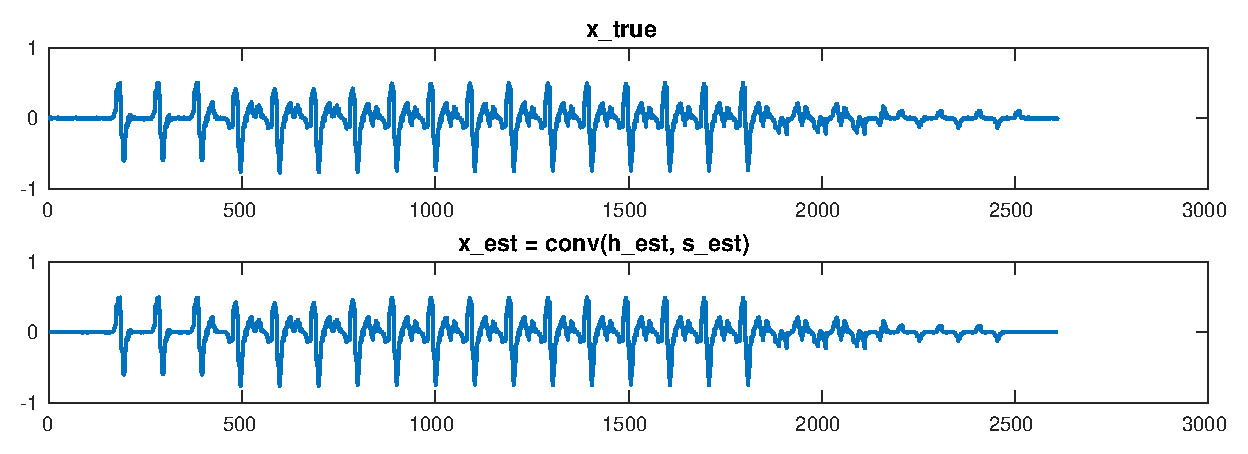
\includegraphics[width=0.5\textwidth]{figures/bce_rec_003_x_trim.pdf}
   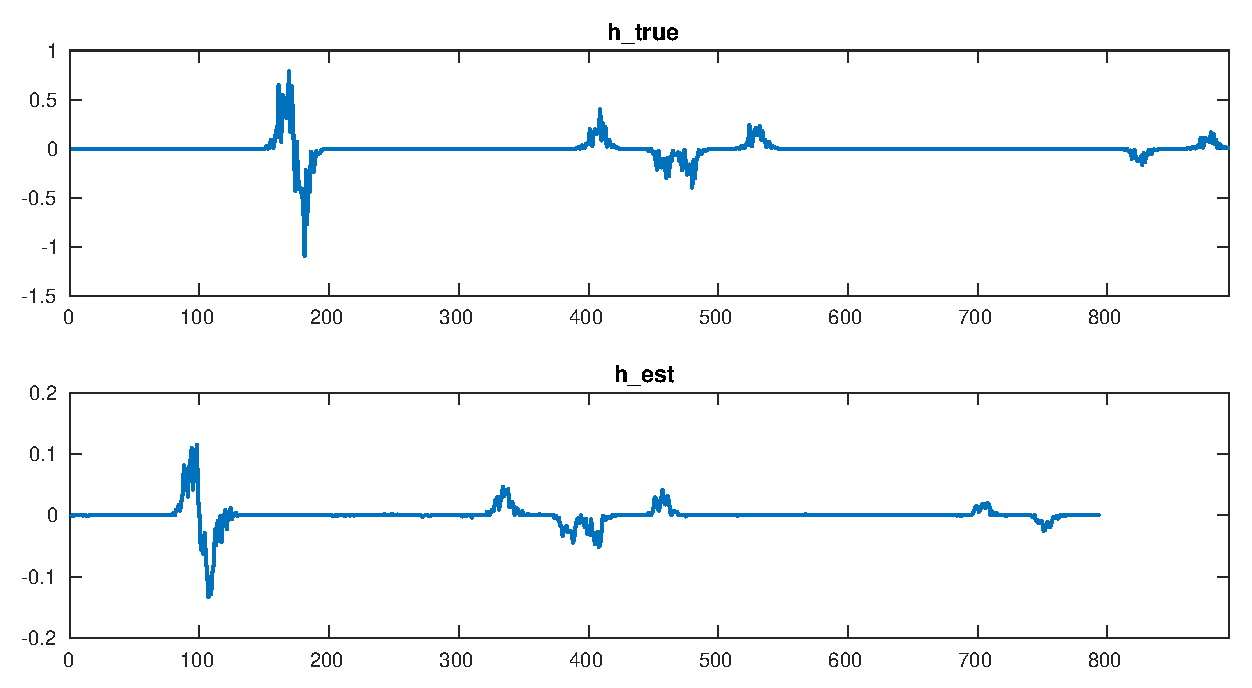
\includegraphics[width=0.5\textwidth]{figures/bce_rec_003_h_trim.pdf}
   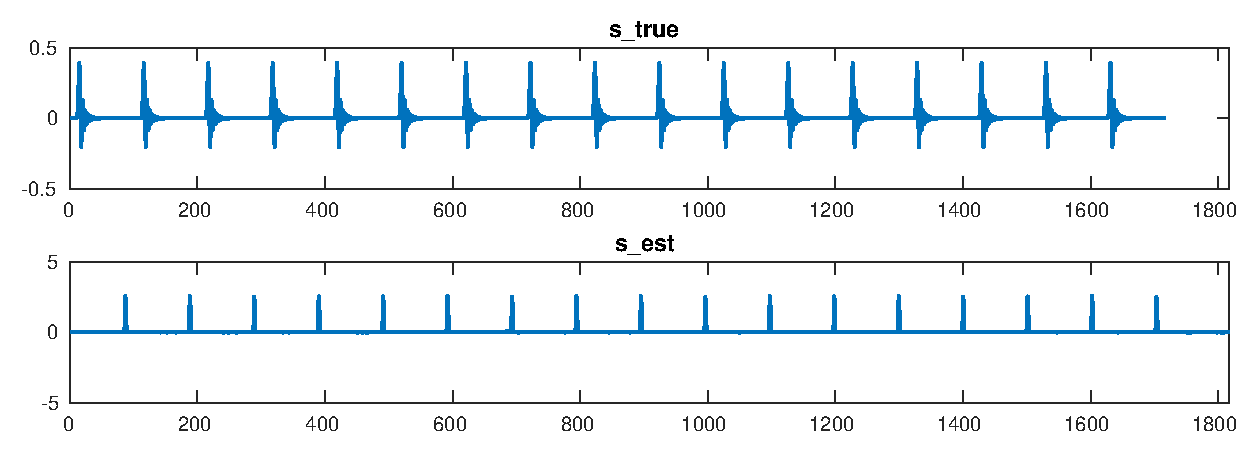
\includegraphics[width=0.5\textwidth]{figures/bce_rec_003_s_trim.pdf}
   \caption{Blind channel estimation via equation (\ref{eq:bce_aug}) for underwater acoustic impulsive source.  We show the impulse response and our estimate for the first of two channels; the second channel is similar.  The recovered source signal and impulse responses appear remarkably similar, with the major differences being a magnitude ambiguity and a time shift.}
   \label{fig:bce_rec}
\end{figure}


% ]]]

\section{Discussion}
% [[[



% ]]]

% References
\bibliographystyle{IEEEtran}
\bibliography{adjoints_in_gradients.bib}

% if you will not have a photo at all:
\begin{IEEEbiographynophoto}{James Folberth}
Biography text here.
\end{IEEEbiographynophoto}

% if you will not have a photo at all:
\begin{IEEEbiographynophoto}{Stephen Becker}
Biography text here.
\end{IEEEbiographynophoto}

\end{document}

% vim: set spell:
% vim: foldmarker=[[[,]]]
